%%%%%%%%%%%%%%%%%%%%%%%%%%%%%%%%%%%%%%%%%%%%%%%%%%%%%%%%%%%%
\documentclass[9pt,            % Schriftgröße {{{
               a4paper,         % A4
               landscape,
               halfparskip,
               oneside,         % Einseitig
               DIV94,           % Papiergröße
              ]{scrartcl} %%% }}}
%%%%%%%%%%%%%%%%%%%%%%%%%%%%%%%%%%%%%%%%%%%%%%%%%%%%%%%%%%%%

%%%%%%%%%%%%%%%%%%%%%%%%%%%%%%%%%%%%%%%%%%%%%%%%%%%%%%%%%%%%
%%% Pakete {{{
\usepackage[utf8]{inputenc}         % Umlaute etc.
\usepackage[T1]{fontenc}            % T1-kodierte Fonts
\usepackage{ae,aecompl}             % Kodierung für PDF
\usepackage{ngerman}                % Deutsche Trennungen,
                                    % dt. Begriffe
\usepackage{setspace}               % Single- oder Onehalfspacing
\setcounter{tocdepth}{4}            % 4 Hirarchien im Inhaltsv.
\usepackage{times}                  % Times als Schrift
\usepackage{amsmath,amssymb,amstext}% Mathematische Symbole
\usepackage{exscale}                % Skalierung von Summen-c und Int.-zeichen
\usepackage{url}                    % Darstellung von URLs
\usepackage{calc}

%%% Optional, je nach Dokument
% \usepackage{listings}             % Quelltext-Listings
% \usepackage{units}                % Technische Units
% \usepackage{psfrag}               % Ersetzts PS-Schriften
  \usepackage{color}                % Farben in LaTeX
% \usepackage{floatflt}             % Textumflossene Bilder...
% \usepackage{picins}               % Textumflossene Bilder
  \usepackage{textcomp}             % Spezielle Zeichen
  \usepackage{gensymb}              % Spezielle Zeichen
% \usepackage{eurosym}              % Euro-Symbol
% \usepackage{currvita}             % Befehle für CVs
  \usepackage{ifpdf}                % Wird ein PDF erstellt?

%%% Layout
\usepackage{scrpage2}               % KOMA-Überschriften und -Fußzeilen.
%%% }}}
%%%%%%%%%%%%%%%%%%%%%%%%%%%%%%%%%%%%%%%%%%%%%%%%%%%%%%%%%%%%

%%%%%%%%%%%%%%%%%%%%%%%%%%%%%%%%%%%%%%%%%%%%%%%%%%%%%%%%%%%%
%%% PDF {{{

\ifpdf
  \usepackage[pdftex]{graphicx}
  \DeclareGraphicsExtensions{.pdf}
  \pdfcompresslevel=9
  \usepackage[%
    pdftex=true,
    backref=true,
    colorlinks=true,
    bookmarks=true,
    breaklinks=true,
    linktocpage=true,
    bookmarksopen=false,
    bookmarksnumbered=false,
    pdfpagemode=None
  ]{hyperref}
  \hypersetup{
    pdftitle={},
    pdfauthor={Julius Plenz},
    pdfsubject={},
    pdfcreator={LaTeX2e and pdfLaTeX},
    pdfproducer={},
    pdfkeywords={}
  }
\else
  \usepackage[dvips]{graphicx}
  \DeclareGraphicsExtensions{.eps}
  % \usepackage[%
  %   dvips,
  %   breaklinks=true,
  %   colorlinks=false
  % ]{hyperref}
\fi

%%% }}}
%%%%%%%%%%%%%%%%%%%%%%%%%%%%%%%%%%%%%%%%%%%%%%%%%%%%%%%%%%%%

%%%%%%%%%%%%%%%%%%%%%%%%%%%%%%%%%%%%%%%%%%%%%%%%%%%%%%%%%%%%
%%% Eigene Funktionen {{{
%%% Beispiel:  \bild{200pt}{foo}{That's a foo\ldots}
\newcommand{\bild}[3]{
  \begin{figure}
    \includegraphics[width=#1, keepaspectratio=true]{#2}
    \caption{#3}
    \label{#2}
  \end{figure}
}

%% \floatimg{filename}{caption+label}{r/l}{8cm}
\newcommand{\floatimg}[4]{
  \piccaption{#2}
  \parpic[#3]{\includegraphics[width=#4]{#1}}
}

\newcommand{\platz}{\vspace{-4.5ex}}

%%% }}}
%%%%%%%%%%%%%%%%%%%%%%%%%%%%%%%%%%%%%%%%%%%%%%%%%%%%%%%%%%%%

%%%%%%%%%%%%%%%%%%%%%%%%%%%%%%%%%%%%%%%%%%%%%%%%%%%%%%%%%%%%
%%% Pagestyle {{{
% \pagestyle{scrheadings}
% \pagestyle{fancyhdrs}
  \pagestyle{empty}
%%% }}}
%%%%%%%%%%%%%%%%%%%%%%%%%%%%%%%%%%%%%%%%%%%%%%%%%%%%%%%%%%%%

%%%%%%%%%%%%%%%%%%%%%%%%%%%%%%%%%%%%%%%%%%%%%%%%%%%%%%%%%%%%
%%% Seitenkopf- und -Fußzeilen {{{
 \automark[subsection]{section} % \left- und \rightmark bekommen Inhalt
%%% Oben: Links, Mitte, Rechts
 \ihead[]{}
 \chead[]{}
 \ohead[]{}
%%% Unten: Links, Mitte, Rechts
 \ifoot[]{}
 \cfoot[]{}
 \ofoot[]{}
%%% }}}
%%%%%%%%%%%%%%%%%%%%%%%%%%%%%%%%%%%%%%%%%%%%%%%%%%%%%%%%%%%%

\usepackage{tikz}
\usetikzlibrary{shapes,decorations,shadows}

%%%%%%%%%%%%%%%%%%%%%%%%%%%%%%%%%%%%%%%%%%%%%%%%%%%%%%%%%%%%
%%% Sonstiges {{{
% \setlength{\parindent}{17pt}      % Einzug 17pt,
% \setlength{\parskip}{2pt}         % keine Leerzeilen.

% \textwidth      127mm             % Textbreite
% \textheight     235mm             % Texthöhe
% \topmargin     -5mm               % Abstand oben
% \oddsidemargin  7mm               % Abstand Links, onepage

%\onehalfspacing                    % Zeilenabstand: Bei korrektur,
 \singlespacing                     % bei Abgabe

% Punkt- und Komma Abstände bei Tausendern/
% Dezimalzahlen ans deutsche anpassen!
 \mathcode`,="013B
 \mathcode`.="613A

 \setlength{\emergencystretch}{2em} % Notfallsstreckung
 \addtolength{\voffset}{10pt}

% Kommandoänderungen
 \renewcommand{\figurename}{Abb.} % Bildunterschriften: Abb. anstatt Fig.
%\renewcommand*{\cvheadingfont}{\raggedleft\Huge\bfseries} % CV: Überschriften
%%% }}}
%%%%%%%%%%%%%%%%%%%%%%%%%%%%%%%%%%%%%%%%%%%%%%%%%%%%%%%%%%%%


% Platz links, über und unter Überschriften ändern
%\usepackage{titlesec}
%\titlespacing*{\subsection}{0pt}{5.5ex plus 1ex minus .2ex}{4.3ex plus .2ex}


\begin{document}

%%%%%%%%%%%%%%%%%%%%%%%%%%%%%%%%%%%%%%%%%%%%%%%%%%%%%%%%%%%%
%%% Inhalt {{{


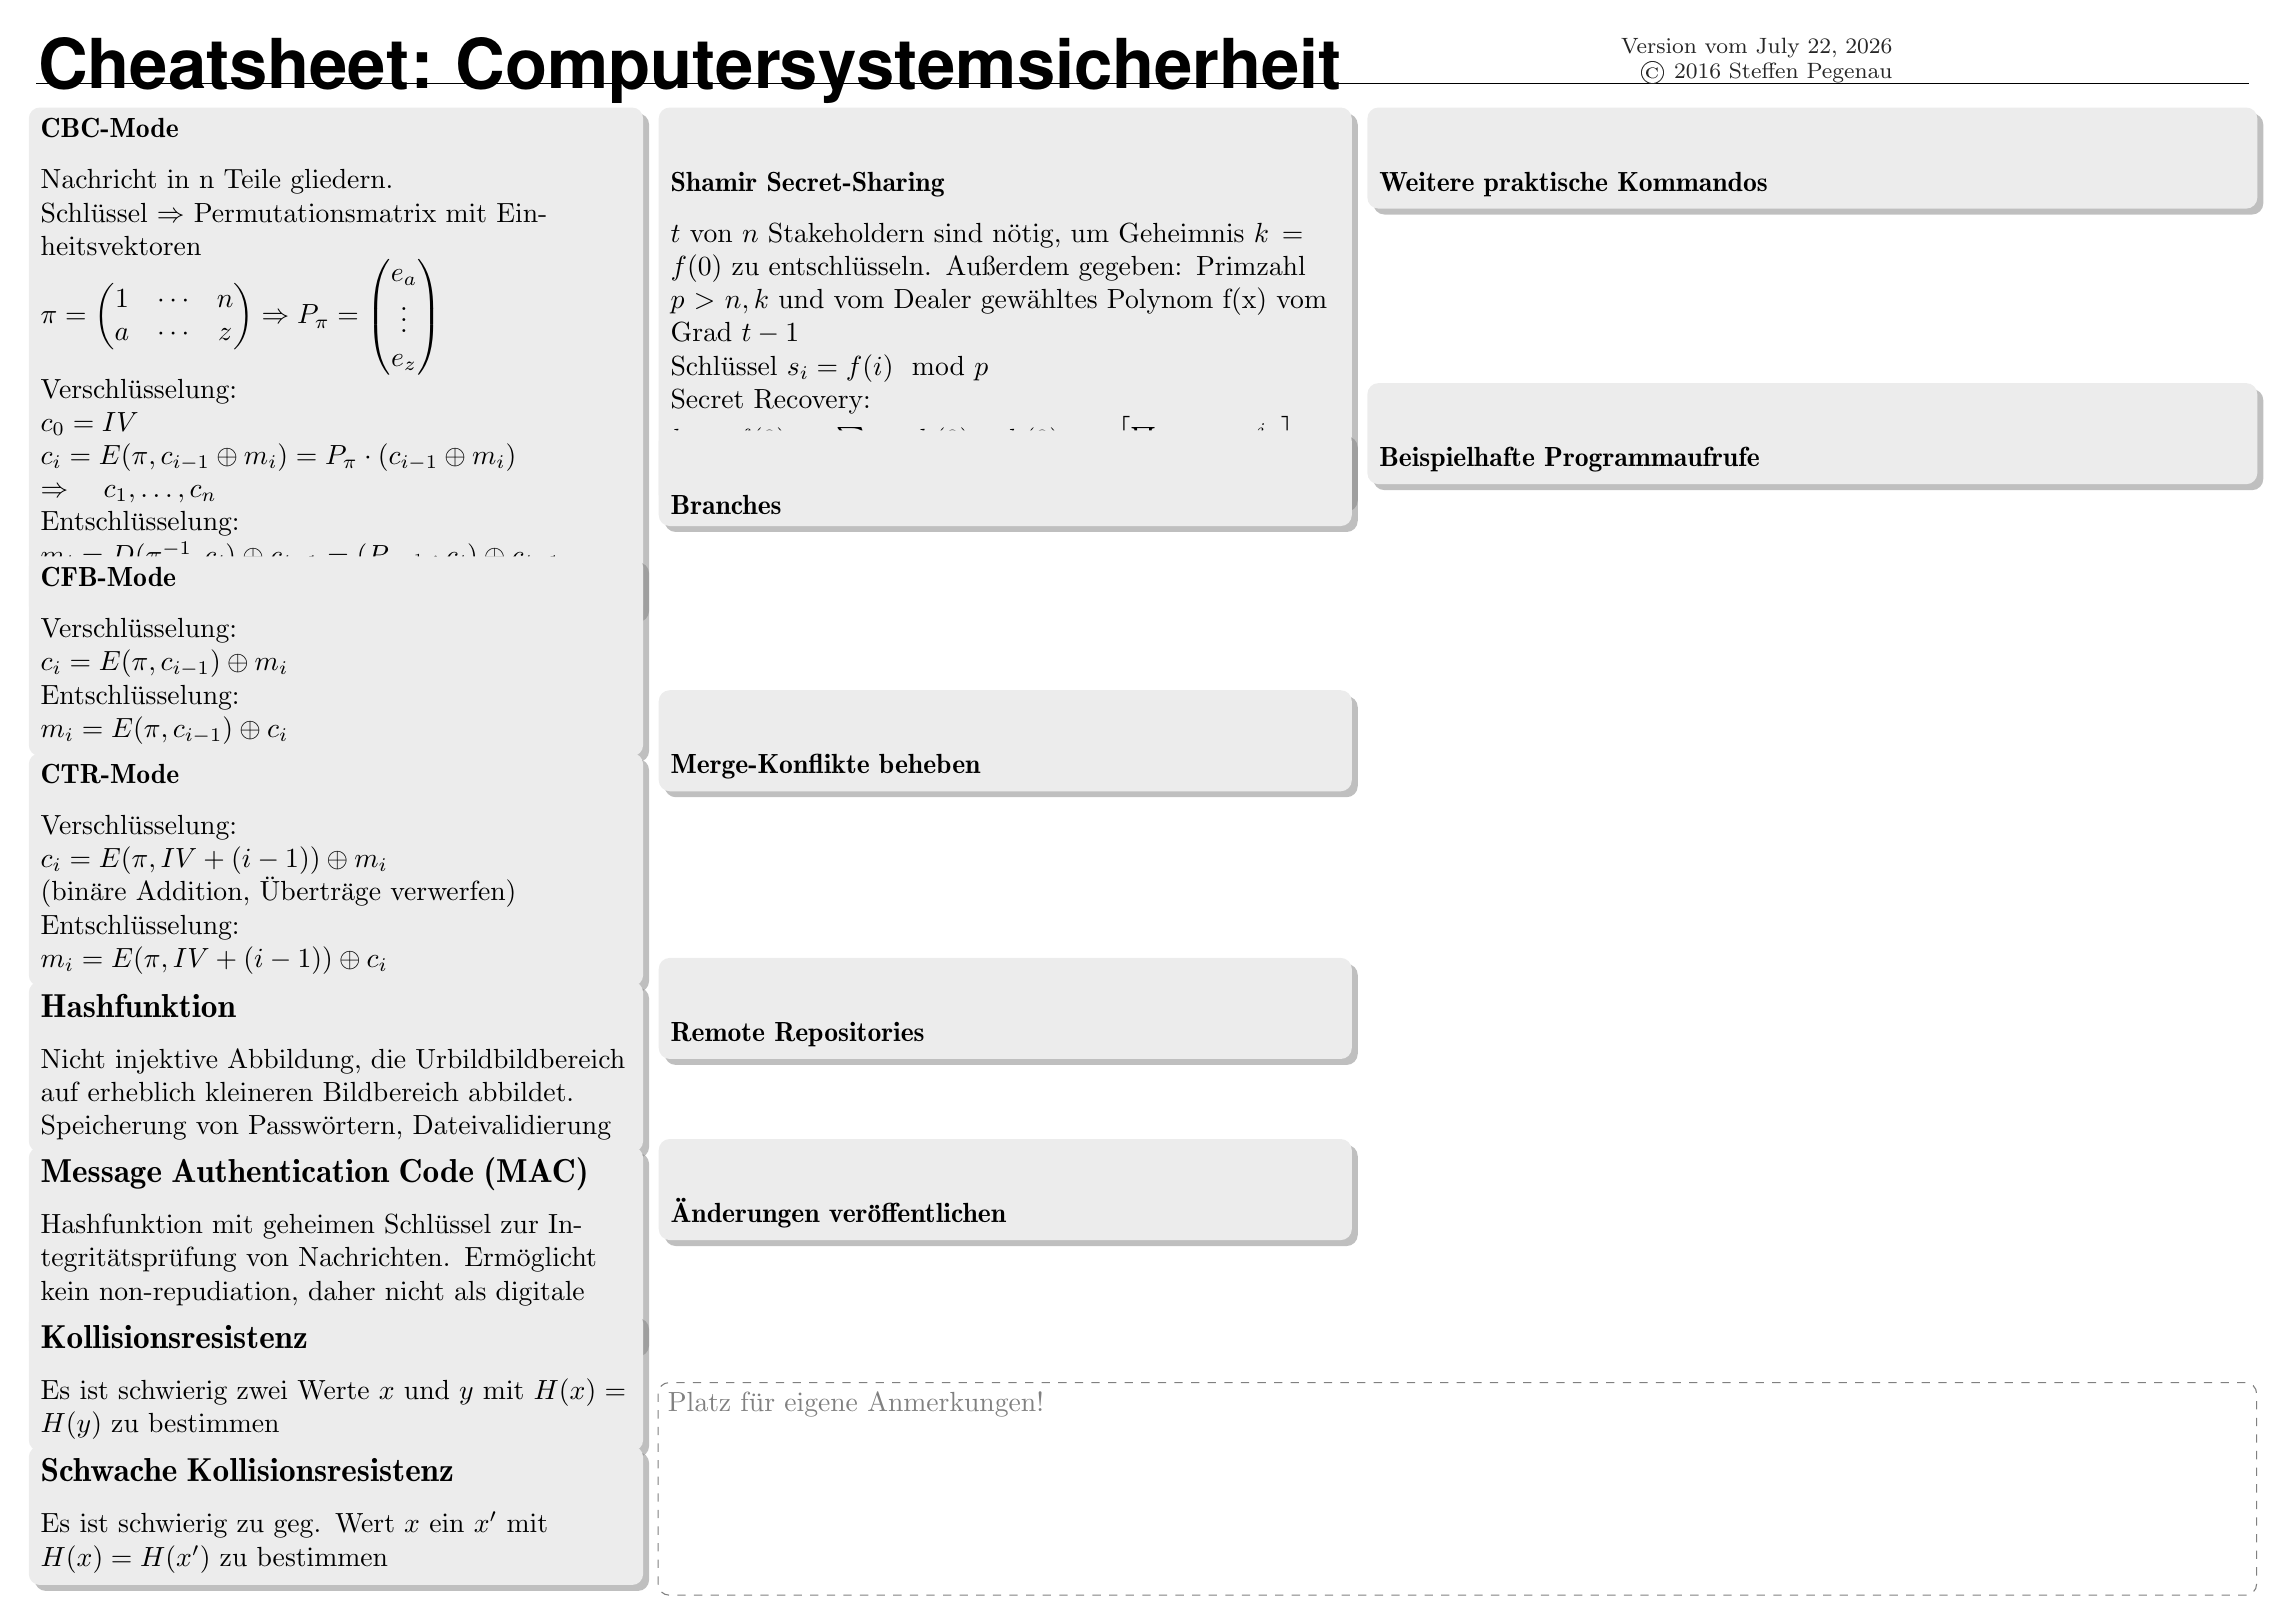
\begin{tikzpicture}
  \draw (0,1) node[anchor=north west,font=\Huge\bf\fontfamily{phv}\selectfont]{Cheatsheet: Computersystemsicherheit}
  (.1cm,.3cm) -- (28.2cm,.3cm)
  ([xshift=1mm]23.7cm,.7cm)
  node[font=\footnotesize,color=black!85,anchor=north east]{
    \copyright{} 2016 Steffen Pegenau
  }
  ++(0,.3cm)
  node[font=\footnotesize,color=black!85,anchor=north east]{
    Version vom \today
  }
  ;
  \draw
  (0,0) node[anchor=north west,text width=7.5cm,rounded corners,fill=gray!15,inner sep=1ex,drop shadow]
  (linksoben)
  {
   \platz
   \subsubsection*{CBC-Mode}
    Nachricht in n Teile gliedern. \\
    Schlüssel $\Rightarrow$ Permutationsmatrix mit Einheitsvektoren\\
    $\pi = \left(
    \begin{matrix}
     1 & \cdots & n \\
     a & \cdots & z \\
    \end{matrix} \right)
    \Rightarrow
    P_\pi = \left(
    \begin{matrix}
    e_a \\
    \vdots \\
    e_z \\
    \end{matrix}
    \right) $ \\
    Verschlüsselung: \\
    $c_0 = IV$ \\
    $c_i = E(\pi, c_{i-1} \oplus m_i) = P_\pi \cdot (c_{i-1} \oplus m_i)$\\
    $\Rightarrow \quad c_1, \dots, c_n$ \\
    Entschlüsselung: \\
    $m_i = D(\pi^{-1},c_i)\oplus c_{i-1} = (P_{\pi^{-1}} \cdot c_i) \oplus c_{i-1}$\\
    mit $\pi^{-1} = \pi'$ (transponiert)
  }
  ++(0,-5.7cm) node[below right,text width=7.5cm,rounded corners,fill=gray!15,inner sep=1ex,drop shadow]
  {
    \platz
    \subsubsection*{CFB-Mode}
    Verschlüsselung: \\
    $c_i = E(\pi, c_{i-1} )\oplus m_i$\\
    Entschlüsselung: \\
    $m_i = E(\pi, c_{i-1}) \oplus c_i$
  }
  ++(0,-2.5cm) node[below right,text width=7.5cm,rounded corners,fill=gray!15,inner sep=1ex,drop shadow]
  {
    \platz
    \subsubsection*{CTR-Mode}
    Verschlüsselung: \\
    $ c_i = E(\pi, IV + (i-1)) \oplus m_i $ \\
    (binäre Addition, Überträge verwerfen) \\
    Entschlüsselung: \\
    $ m_i = E(\pi, IV + (i-1)) \oplus c_i $
  }
  ++(0, -2.9cm) node[below right,text width=7.5cm,rounded corners,fill=gray!15,inner sep=1ex,drop shadow]
  {
    \platz
    \subsection*{Hashfunktion}
    Nicht injektive Abbildung, die Urbildbildbereich auf erheblich kleineren Bildbereich abbildet.\\
    Speicherung von Passwörtern, Dateivalidierung
    
  }
  ++(0, -2.1cm) node[below right,text width=7.5cm,rounded corners,fill=gray!15,inner sep=1ex,drop shadow]
  {
    \platz
    \subsection*{Message Authentication Code (MAC)}
    Hashfunktion mit geheimen Schlüssel zur Integritätsprüfung von Nachrichten. Ermöglicht 
    kein non-repudiation, daher nicht als digitale Unterschrift geeignet.
  }
  ++(0, -2.1cm) node[below right,text width=7.5cm,rounded corners,fill=gray!15,inner sep=1ex,drop shadow]
  {
    \platz
    \subsection*{Kollisionsresistenz}
    Es ist schwierig zwei Werte $x$ und $y$ mit $H(x) = H(y)$ zu bestimmen
  }
  ++(0, -1.7cm) node[below right,text width=7.5cm,rounded corners,fill=gray!15,inner sep=1ex,drop shadow]
  {
    \platz
    \subsection*{Schwache Kollisionsresistenz}
    Es ist schwierig zu geg. Wert $x$ ein $x'$ mit $H(x) = H(x')$ zu bestimmen
  }
% Als Visualisierung brauchbar?
;
  \draw (linksoben.north west)
  ++(8cm,0) node[anchor=north west,text width=8.5cm,rounded corners,fill=gray!15,inner sep=1ex,drop shadow]
  (zweite-spalte)
  {
    \subsubsection*{Shamir Secret-Sharing}
    $t$ von $n$ Stakeholdern sind nötig, um Geheimnis $k = f(0)$ zu entschlüsseln. Außerdem gegeben:
    Primzahl $p>n,k$ und vom Dealer gewähltes Polynom f(x) vom Grad $t-1$ \\
    Schlüssel $s_i = f(i) \mod p$ \\
    Secret Recovery: \\
    $k = f(0) = \sum s_i \cdot l_i(0)$ \quad
    $l_i(0) := \left[\prod_{i=1,j\neq i} \frac{j}{j - i}\right] \mod p$
  }
  ++(0,-4.1cm) node[below right,text width=8.5cm,rounded corners,fill=gray!15,inner sep=1ex,drop shadow]
  {
    \subsubsection*{Branches}
  }
  ++(0,-3.3cm) node[below right,text width=8.5cm,rounded corners,fill=gray!15,inner sep=1ex,drop shadow]
  {
    \subsubsection*{Merge-Konflikte beheben}
  }
  ++(0,-3.4cm) node[below right,text width=8.5cm,rounded corners,fill=gray!15,inner sep=1ex,drop shadow]
  {
    \subsubsection*{Remote Repositories}
  }
  ++(0,-2.3cm) node[below right,text width=8.5cm,rounded corners,fill=gray!15,inner sep=1ex,drop shadow]
  {
    \subsubsection*{Änderungen veröffentlichen}
  }
  % Eigene Anmerkungen
  [anchor=north west,draw=gray,dashed,rounded corners] ++(0,-3.1cm) rectangle +(20.3cm,-2.7cm)
  ++(0,0) node[color=gray]{Platz für eigene Anmerkungen!}
  ;
  \draw (zweite-spalte.north west)
  ++(9.0cm,0) node[below right,text width=11.0cm,rounded corners,fill=gray!15,inner sep=1ex,drop shadow]
  {
    \subsubsection*{Weitere praktische Kommandos}
  }
  ++(0,-3.5cm) node[below right,text width=11.0cm,rounded corners,fill=gray!15,inner sep=1ex,drop shadow]
  {
    \subsubsection*{Beispielhafte Programmaufrufe}
  }
  ;
\end{tikzpicture}


%%% }}}
%%%%%%%%%%%%%%%%%%%%%%%%%%%%%%%%%%%%%%%%%%%%%%%%%%%%%%%%%%%%

\end{document}

%%% vim:set fdm=marker:
